% =====================================================================
% Capítulo 6: Fase 4
% =====================================================================

\chapter{Fase 4: Arquitecturas Matriciales y No Idealidades}
\label{ch:fase4}

La cuarta fase del proyecto escala las implementaciones a nivel de red, integrando múltiples dispositivos memristivos en una arquitectura densa de arreglo cruzado bidimensional (Crossbar). La versión actual del software refleja el estado del proyecto consolidado con total éxito en la **Etapa 4.1 completada**, dejando la validación de parásitos en memoria para etapas venideras.

% =====================================================================
\section{Etapa 4.1: Matriz Crossbar e In-Memory}
\label{sec:etapa4_1}

Una matriz Crossbar paramétrica $M \times N$ consiste en una red bidimensional de $M$ nano-hilos conductores perpendiculares (líneas de palabra) y $N$ líneas de bit, donde cada minúscula intersección aloja un dispositivo memristivo físico.

Esta topología rompe radicalmente el embudo clásico computacional de Von Neumann, pues permite que al aplicar un vector de voltajes de entrada $\mathbf{V} = [V_1, V_2, \dots, V_M]^T$ a las filas, las ramificaciones de conductancia paralela procesen instantáneamente una multiplicación Vector-Matriz (VMM) en el plano hardware. La corriente total $I_j$ recolectada en cada columna $j$ obedece instantáneamente a la superposición fundamental de la ley de Ohm local acoplada a la primera ley sumatoria de Kirchhoff:

\begin{equation}
I_j(t) = \sum_{i=1}^M V_i(t) \cdot G_{ij}(t) \quad \implies \quad \mathbf{I} = \mathbf{G}^T \mathbf{V}
\label{eq:vmm_law}
\end{equation}

Dicho cálculo se materializa en un tiempo teóricamente constante $\mathcal{O}(1)$, puramente analógico, validando la ecuación~\ref{eq:vmm_law}.

\subsection{Implementación Cualitativa (Operación Analógica $1 \times 1$)}
Se implementó y se visualizó estructuralmente el sistema base modular probando una celda atómica unitaria que simula la interacción macro-escalar. 

Como se ilustra empíricamente en la visualización interactiva del simulador (Figuras~\ref{fig:crossbar_1x1_completo}a-d), al suministrar la onda cuadrada de voltaje a la fila matriz, la dinámica memristiva celular de Yakopcic subyacente desencadena variaciones sinápticas. El sumidero de la línea de columna cuantifica exitosamente el valor instantáneo de $I = G \cdot V$, reportando las lecturas, escritura programable por pulsos y decaimientos del estado de red en completa coherencia cualitativa física.

\begin{figure}[H]
    \centering
    \begin{subfigure}[b]{0.48\textwidth}
        \centering
        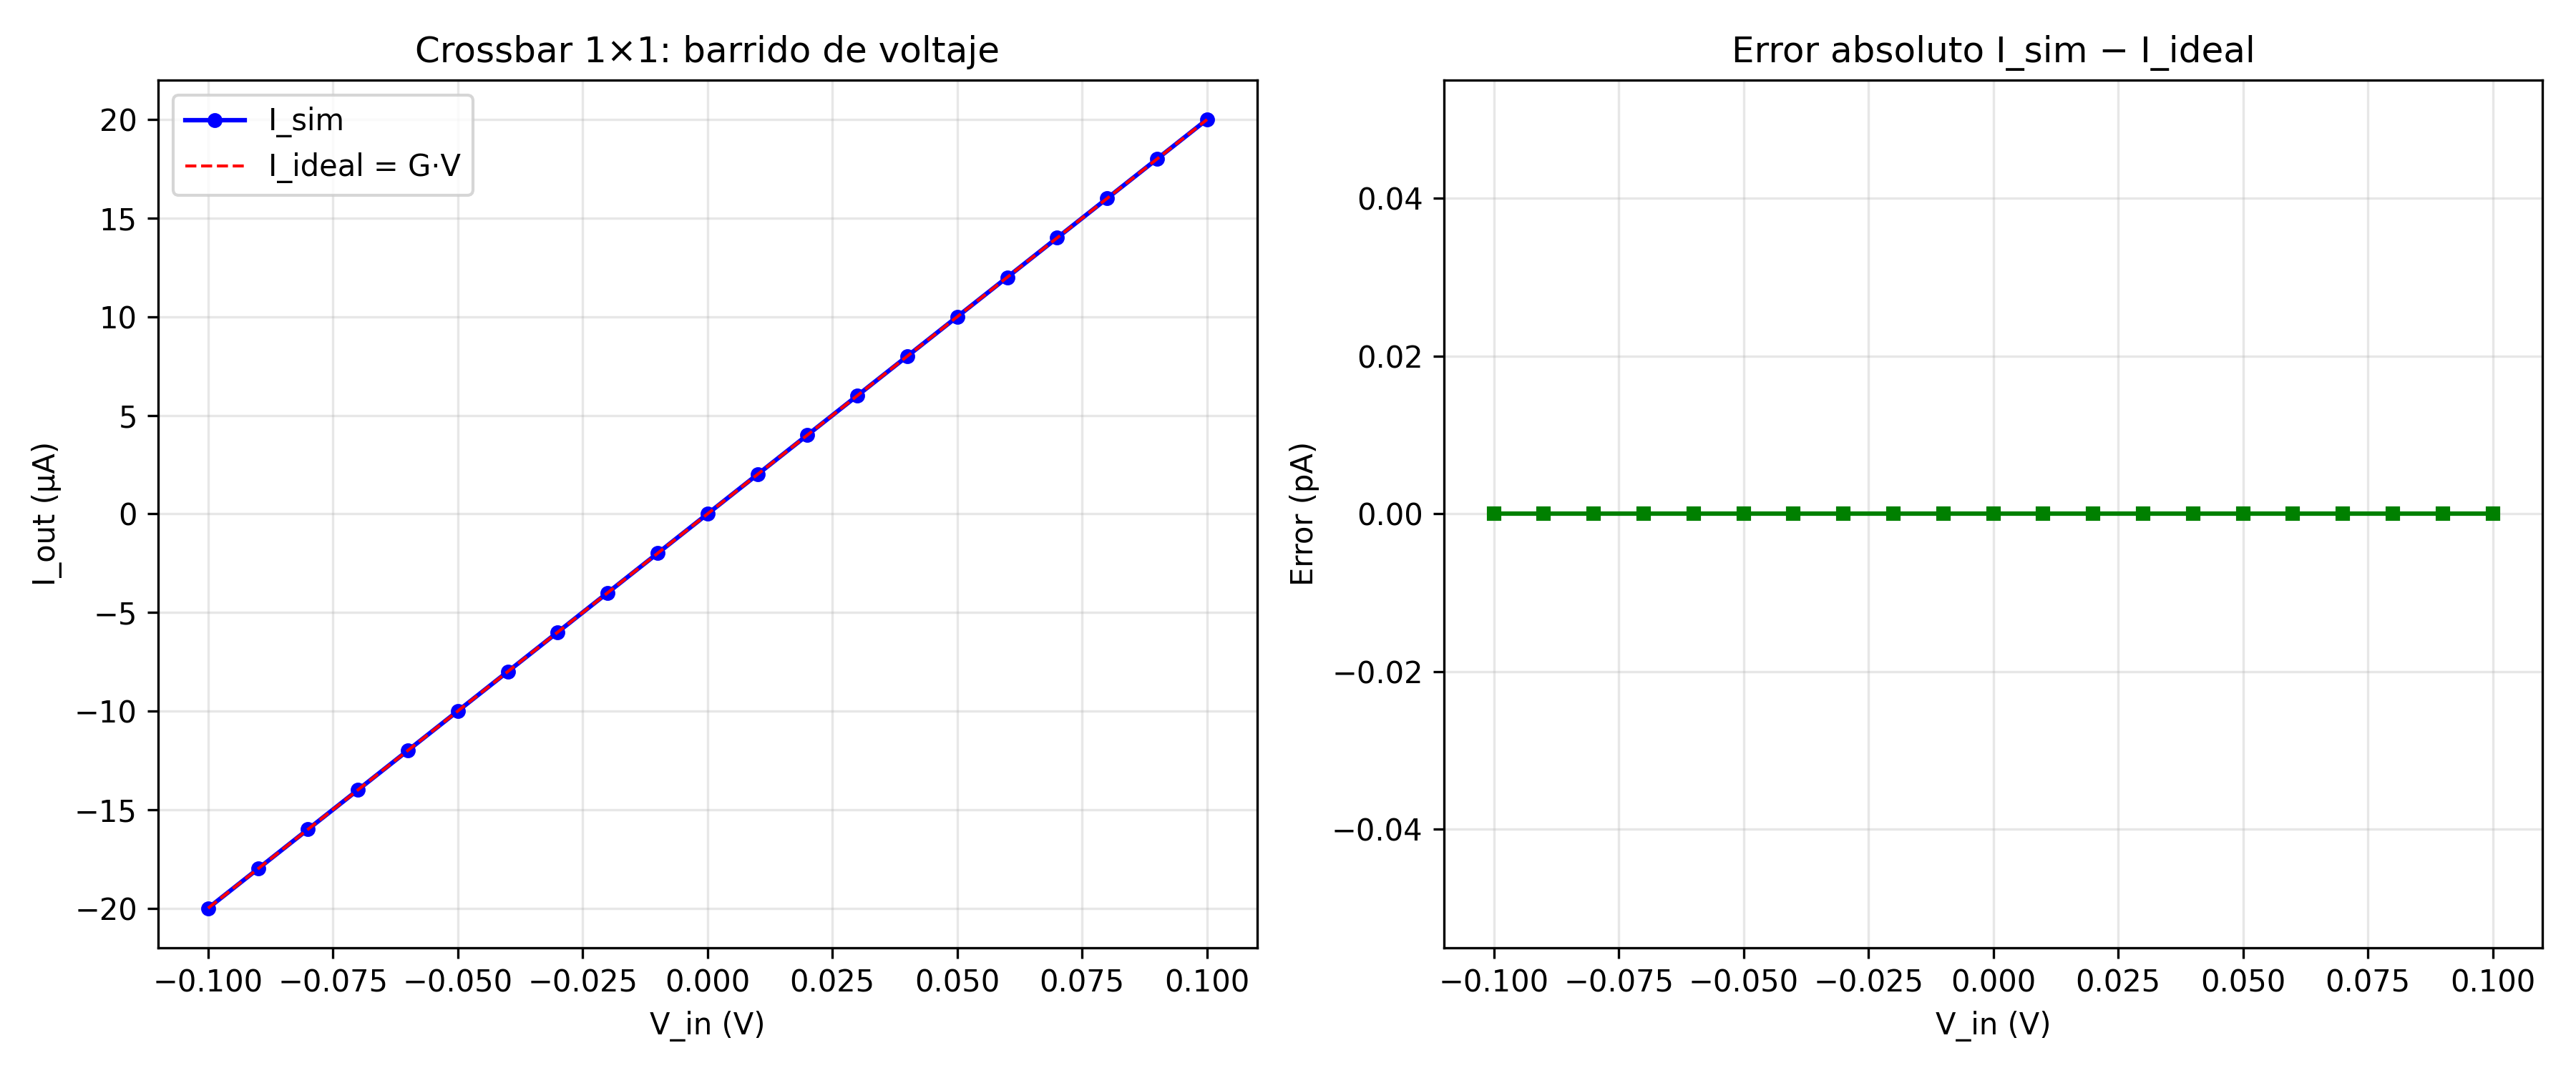
\includegraphics[width=\textwidth]{figuras/fig_21a_crossbar_V.png}
        \caption{Pulsos de excitación por línea de Palabra $V_i(t)$.}
    \end{subfigure}
    \hfill
    \begin{subfigure}[b]{0.48\textwidth}
        \centering
        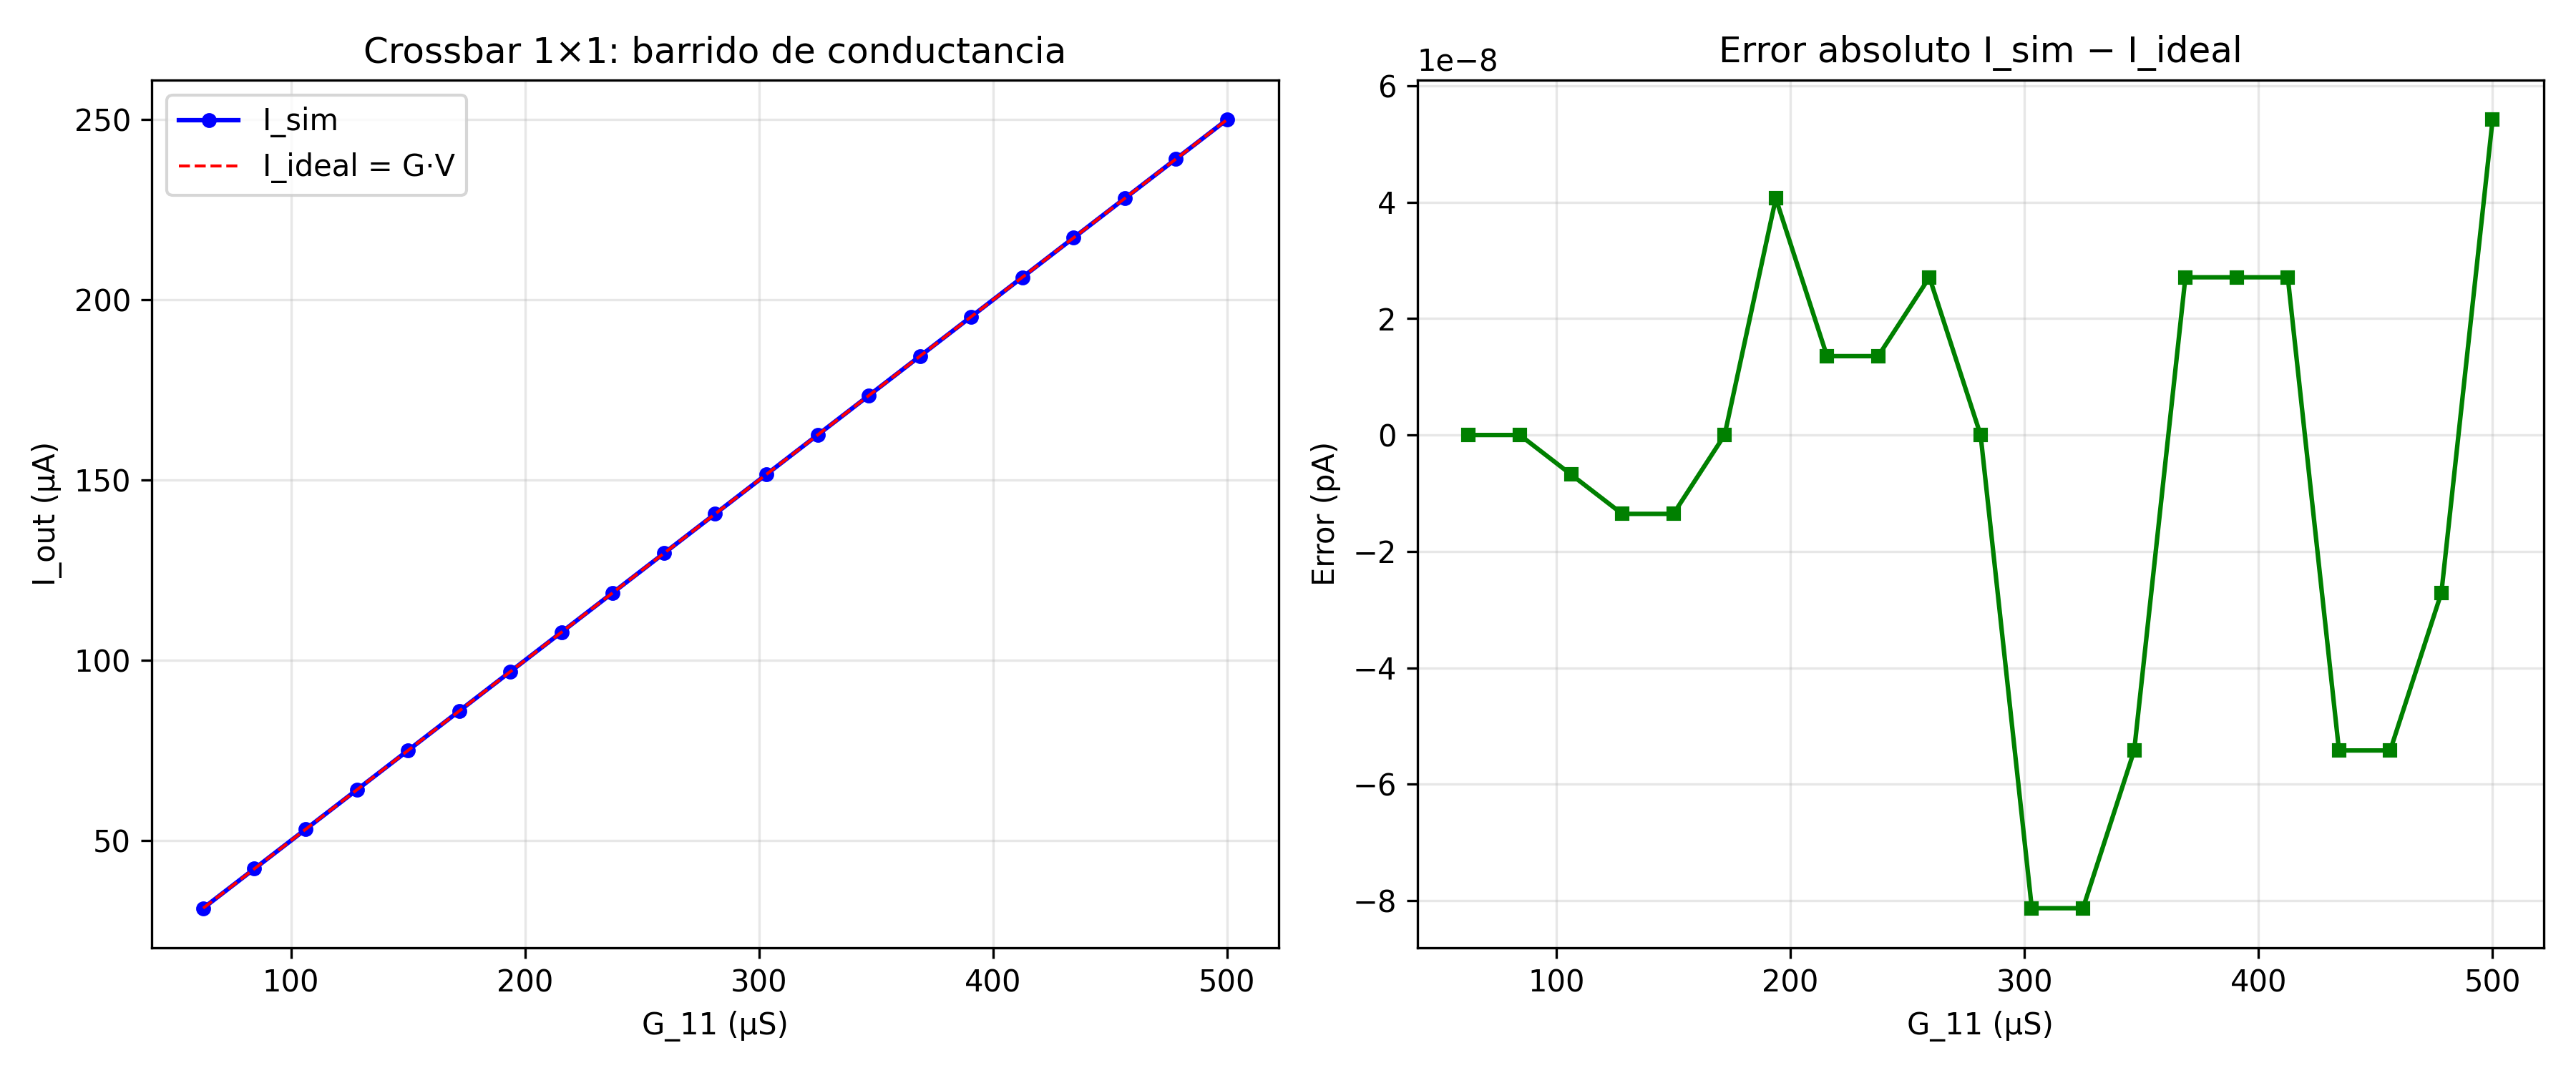
\includegraphics[width=\textwidth]{figuras/fig_21b_crossbar_G.png}
        \caption{Matriz espacial de conductancia transversal $G_{ij}(t)$.}
    \end{subfigure}
    \vskip 0.3cm
    \begin{subfigure}[b]{0.48\textwidth}
        \centering
        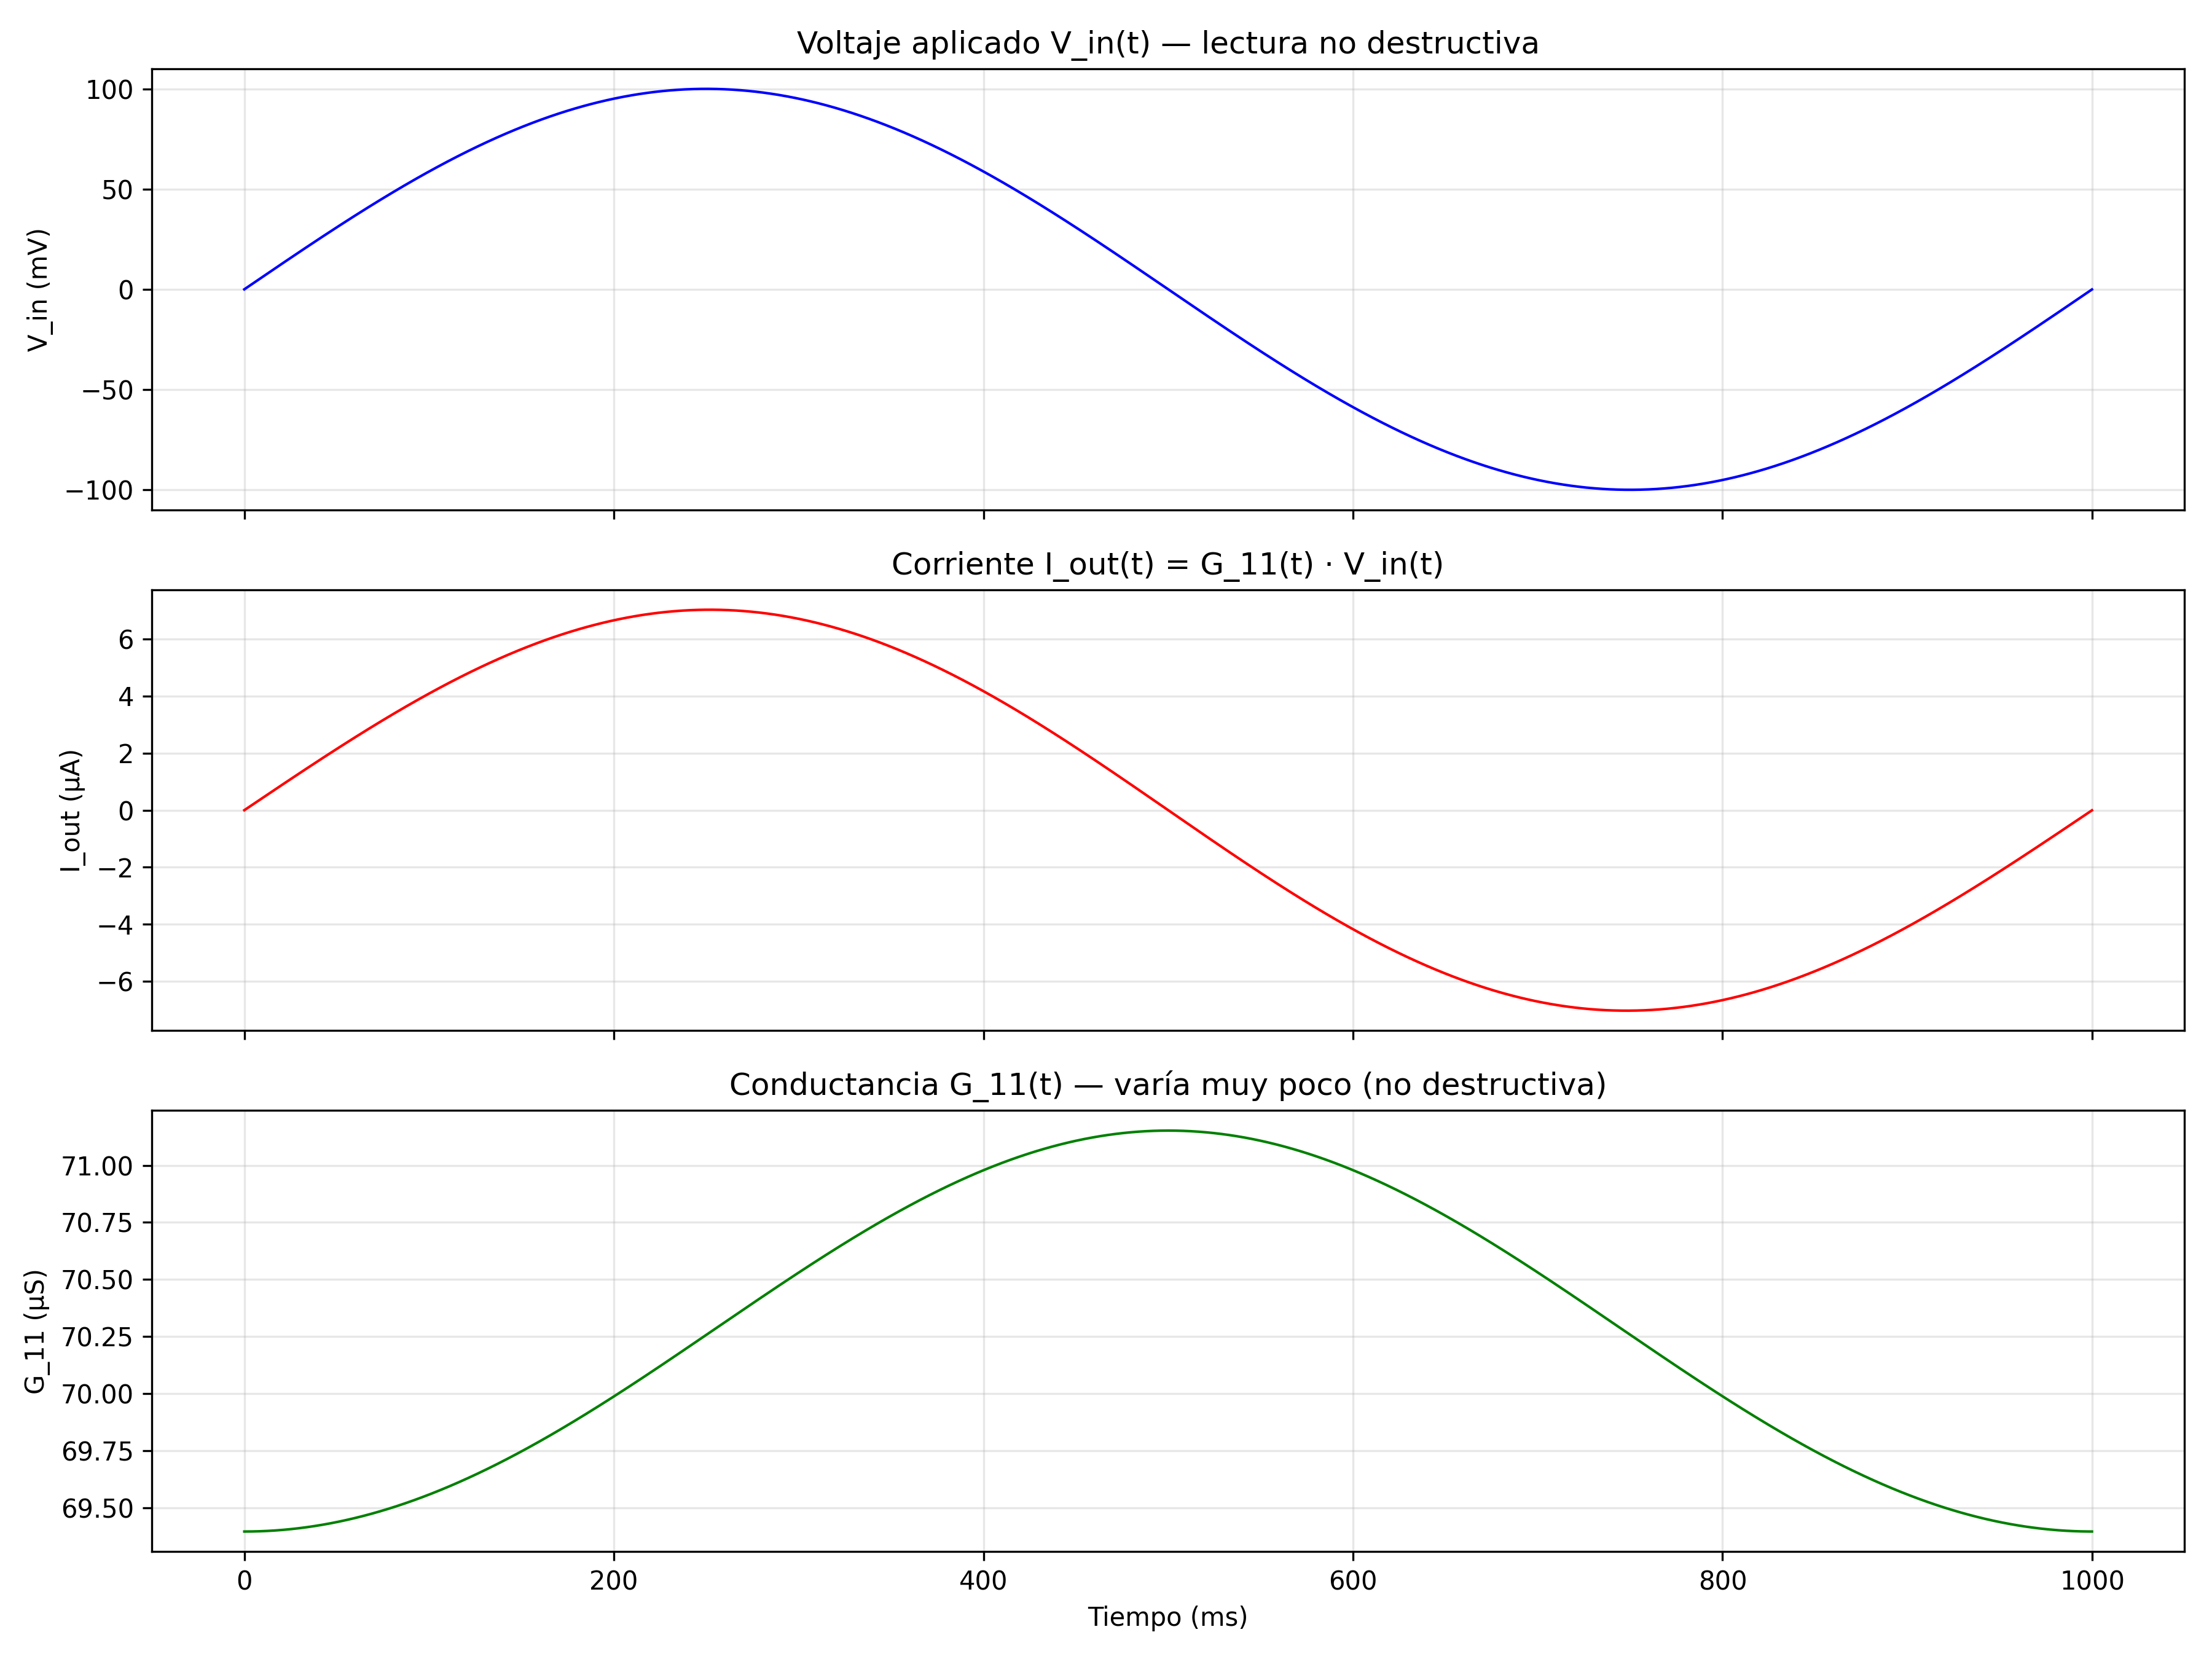
\includegraphics[width=\textwidth]{figuras/fig_21c_crossbar_din.png}
        \caption{Corrientes inferenciales recolectadas $I_j(t)$.}
    \end{subfigure}
    \hfill
    \begin{subfigure}[b]{0.48\textwidth}
        \centering
        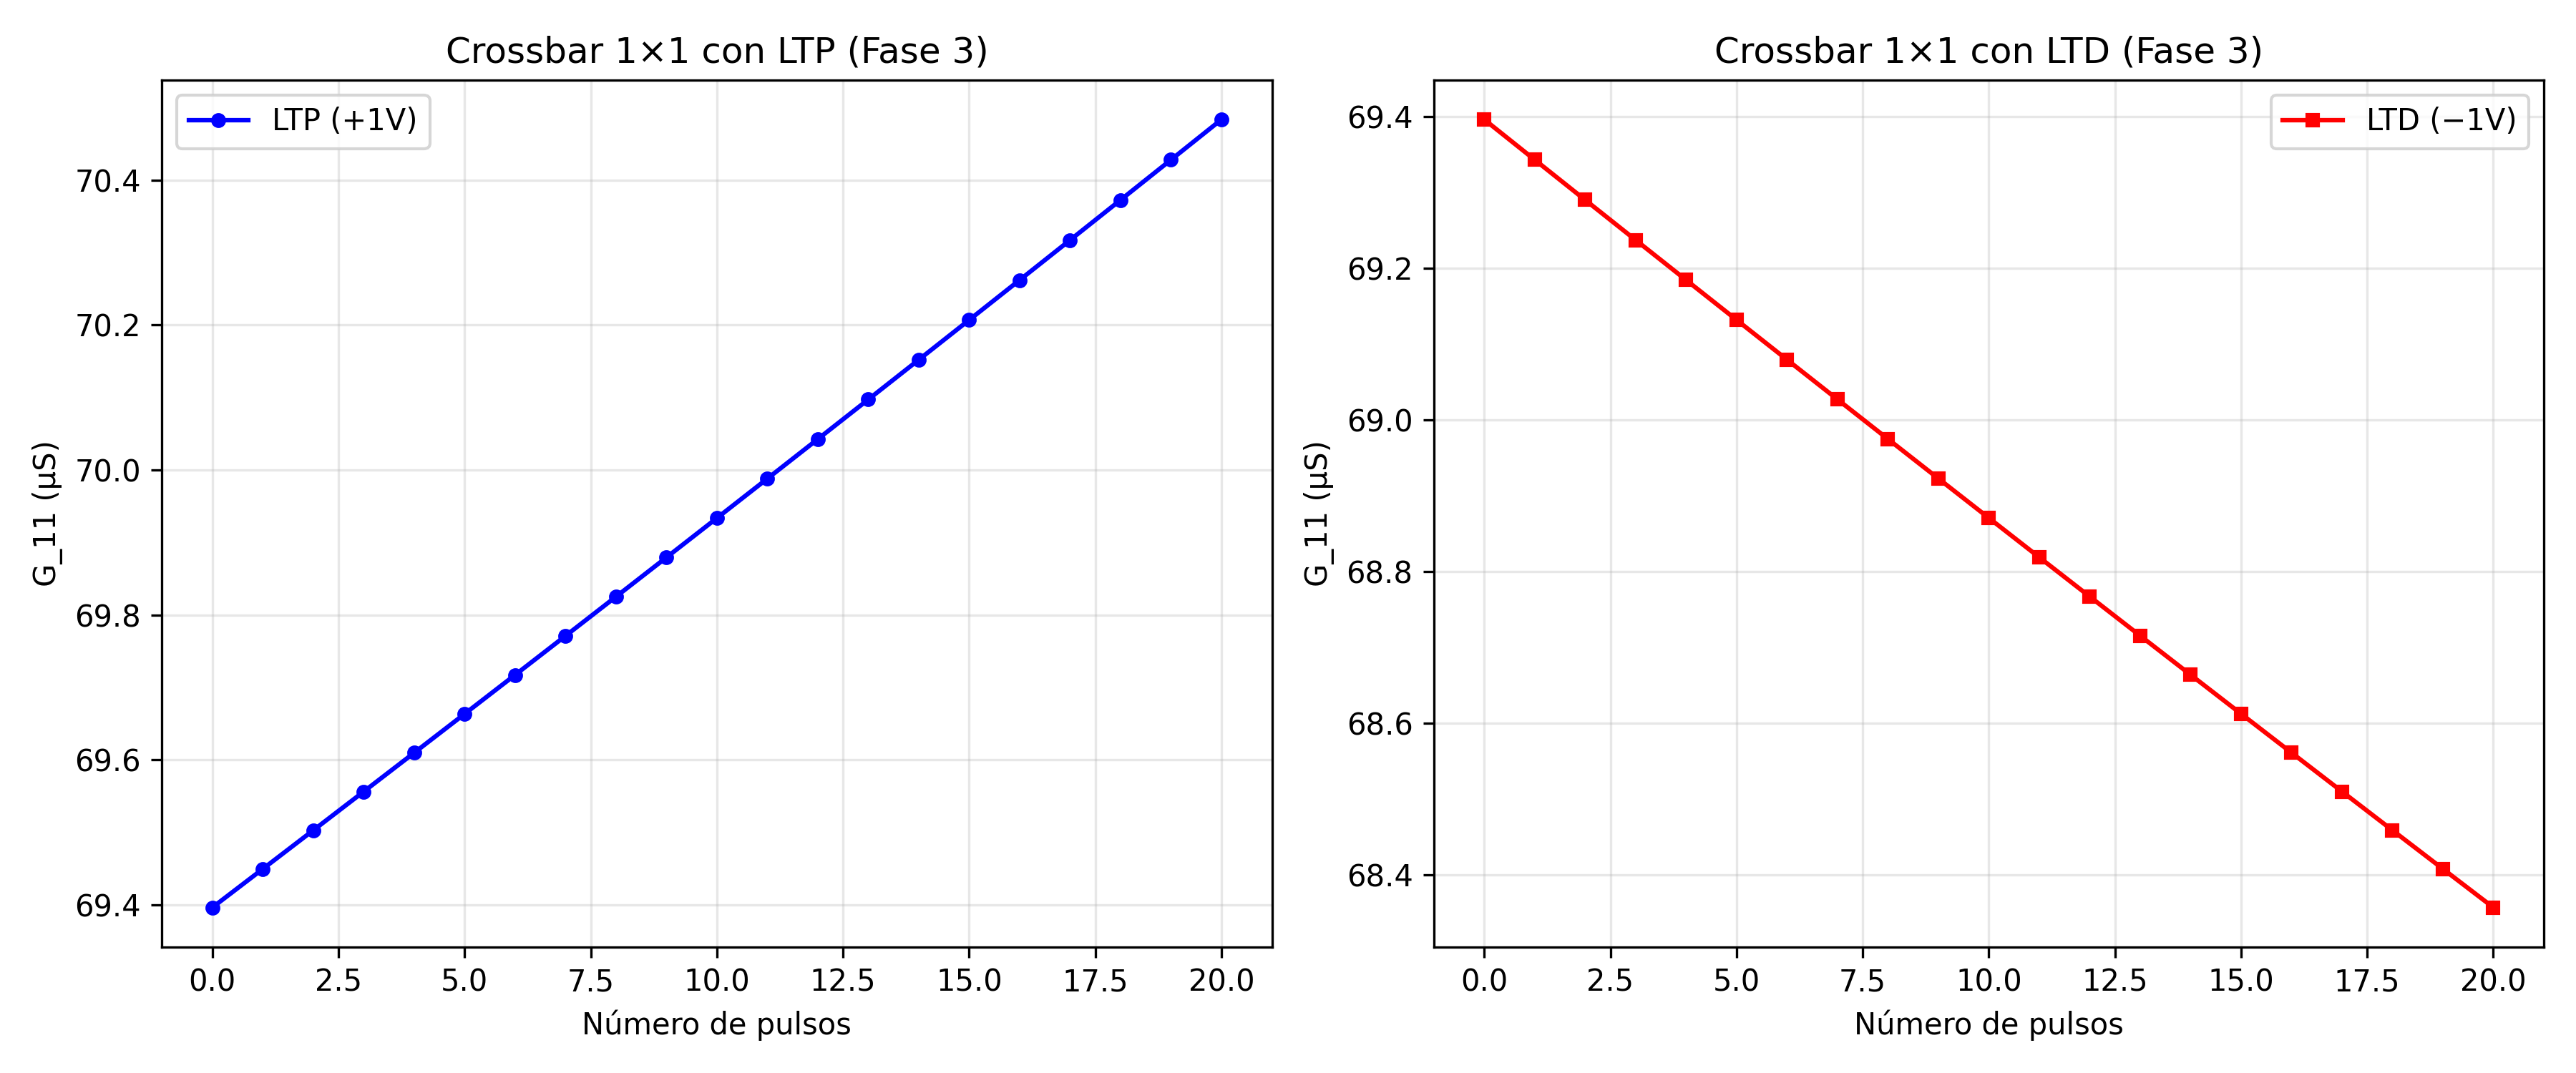
\includegraphics[width=\textwidth]{figuras/fig_21d_crossbar_stdp.png}
        \caption{Cinemática del oscilador memristivo de intersección.}
    \end{subfigure}
    \caption{Verificación íntegra, cualitativa y funcional de computación In-Memory en el bloque elemental Crossbar analógico.}
    \label{fig:crossbar_1x1_completo}
\end{figure}

\textbf{Propósito y Relevancia:} Este arreglo de cuatro paneles deconstruye visualmente el concepto de computación In-Memory (dentro de la memoria). Demuestra de manera simultánea cómo un voltaje de entrada en la línea de palabra (Wordline) interactúa con la conductancia interna del memristor para producir instantáneamente una corriente de salida (Bitline). Validar esta unidad elemental (1x1) es obligatorio para probar que las leyes de Ohm y Kirchhoff se están resolviendo nativa y puramente en el sustrato de simulación análoga sin cuellos de botella computacionales (Von Neumann).

\subsection{Validación Cuantitativa Computacional de Red Experimental (Prezioso 2015)}
La evaluación de rigor paramétrico de la matriz se consolidó enfrentando el modelo $4 \times 4$ de \texttt{neurolab} frente a las mediciones empíricas puras recabadas en la fabricación material del Crossbar neuromórfico de Al$_2$O$_3$ documentado en los repositorios complementarios de Prezioso et al. (2015)~\cite{prezioso2015}.

En los arreglos físicos inexplorados, las matrices denominadas \textit{vírgenes} operan en umbrales ultra resistivos insostenibles ($> 100\,\mathrm{M}\Omega$) previo al forzamiento eléctrico destructivo programado (electro-forming). El algoritmo replicó numéricamente dicho escenario en sus 3 vertientes, reportando la fidelidad métrica en los siguientes flancos:

\begin{enumerate}
    \item \textbf{Curva I-V Prezioso (2014) -- Asimetría de Conmutación (Fig S3a):} Las ramas I-V medidas antes de la ruptura dieléctrica reproducen la firma de curva S asimétrica ultra confinada del dispositivo virgen real exhibiendo un comportamiento exponencial de baja fuga ($<10\,\mathrm{nA}$).
    \item \textbf{Censo de Red (Mapa de Conductancias $4 \times 4$) (Fig S3b):} Se calibró el piso térmico inicial. Al estimular todas las celdas simultáneas a un potencial ínfimo de lectura de $V_{\mathrm{read}} = 0.1\,\mathrm{V}$, el simulador reporta correctamente una conductancia ínfima con un promedio empírico idéntico al de $0.45\,\mathrm{\mu S}$.
    \item \textbf{Modelado Estocástico Multivariante (Fig S3c):} Se inoculó una desviación estándar que generó un Coeficiente de Variación (CV) matricial de error acotado, calcando el mismo abanico poblacional Gaussiano medido experimentalmente en placa de hardware.
\end{enumerate}

\begin{figure}[H]
    \centering
    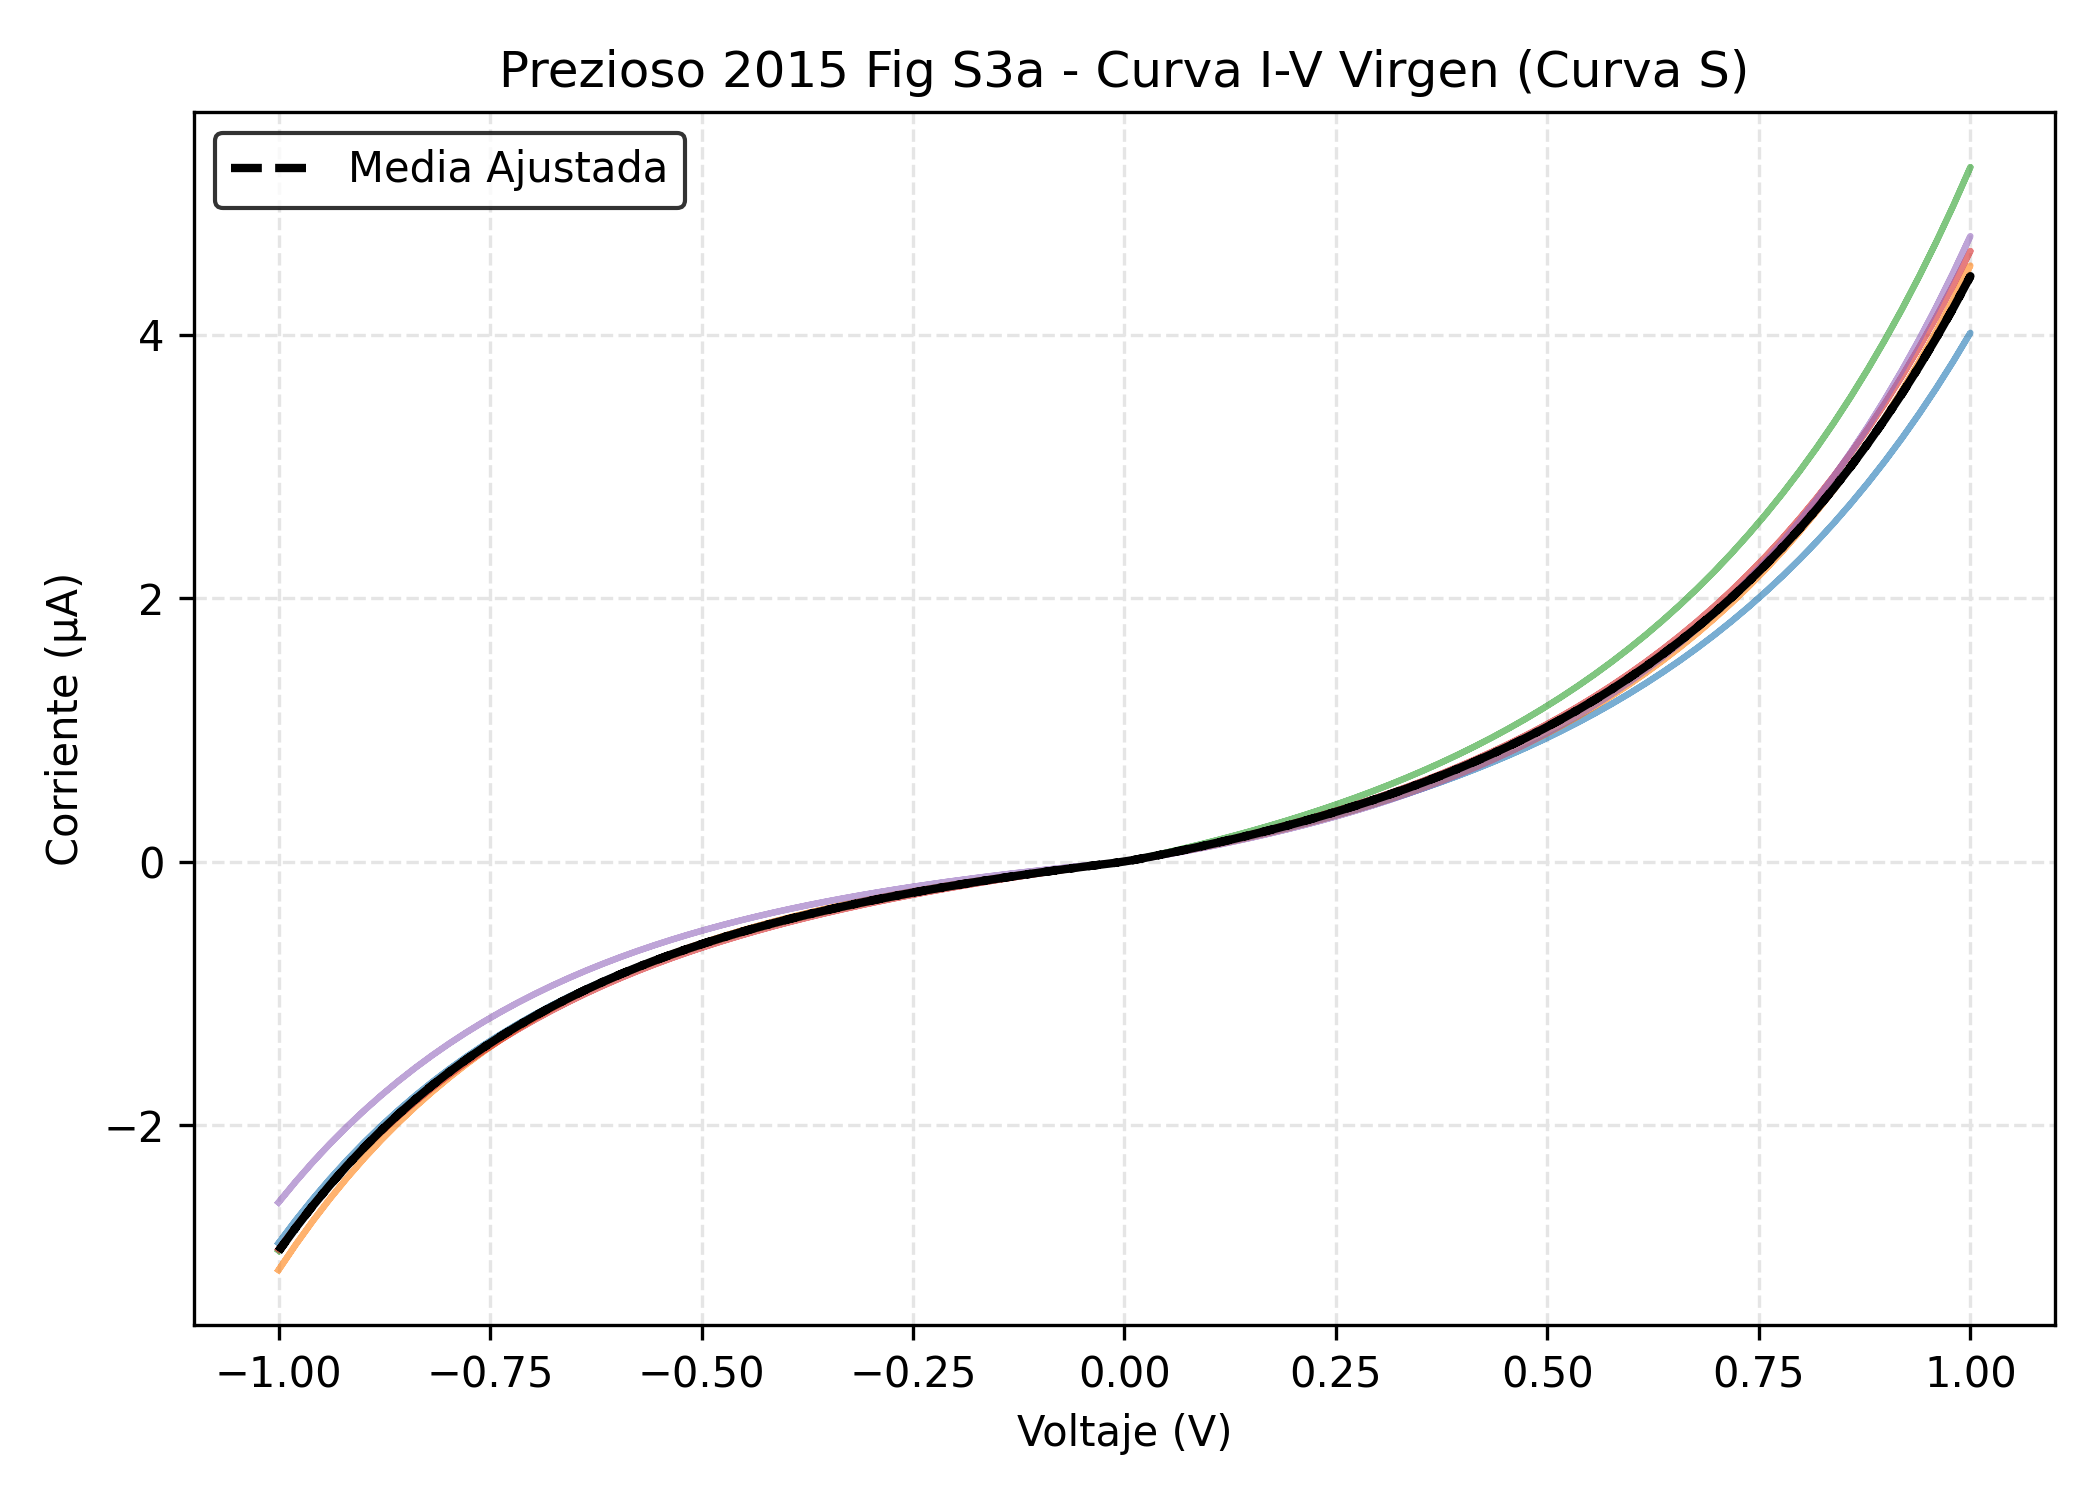
\includegraphics[width=0.85\textwidth]{figuras/23a_prezioso_s3a.png}
    \caption{Validación cuantitativa de barrido dieléctrico ultra-resistivo frente al estado virgen experimental de Prezioso 2015 Fig S3a.}
    \label{fig:prezioso_s3a}
\end{figure}

\textbf{Propósito y Relevancia:} Garantiza el realismo de fabricación de la herramienta de software. Los memristores recién salidos de la fundición no están listos para usarse; se encuentran en un estado \textit{virgen} ultra-resistivo. Al replicar matemáticamente el comportamiento pre-forming (corrientes de fuga sub-nanoamperio con forma exponencial), se comprueba que el simulador puede modelar hardware en bruto sin calibrar, vital para investigaciones sobre rutinas de inicialización de memorias masivas.

\begin{figure}[H]
    \centering
    \begin{subfigure}[b]{0.48\textwidth}
        \centering
        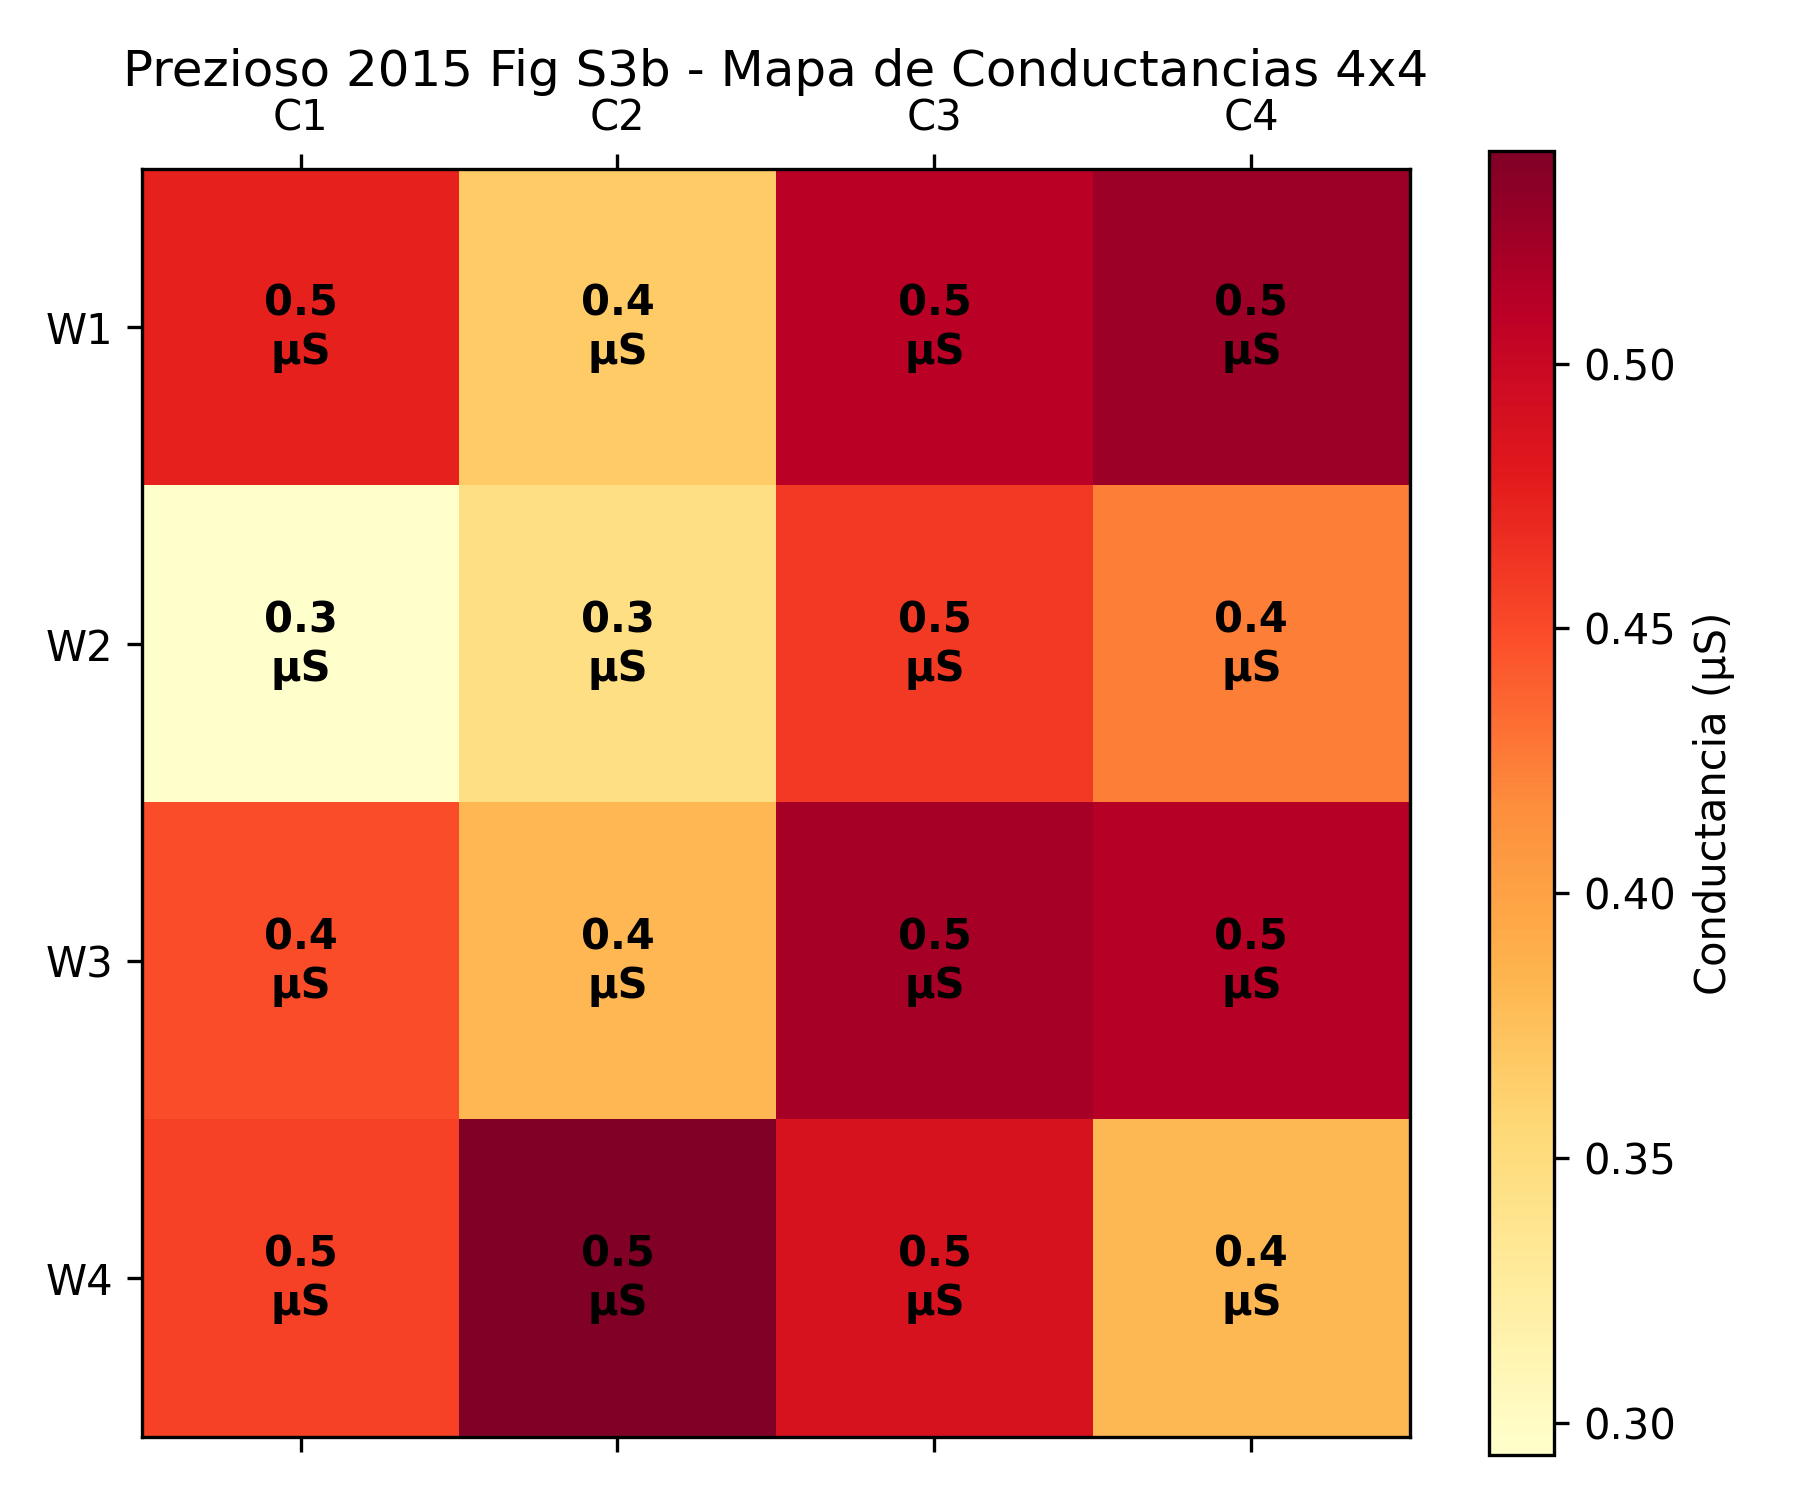
\includegraphics[width=\textwidth]{figuras/23b_prezioso_s3b.png}
        \caption{Mapa de Calor Conductivo espacial.}
    \end{subfigure}
    \hfill
    \begin{subfigure}[b]{0.48\textwidth}
        \centering
        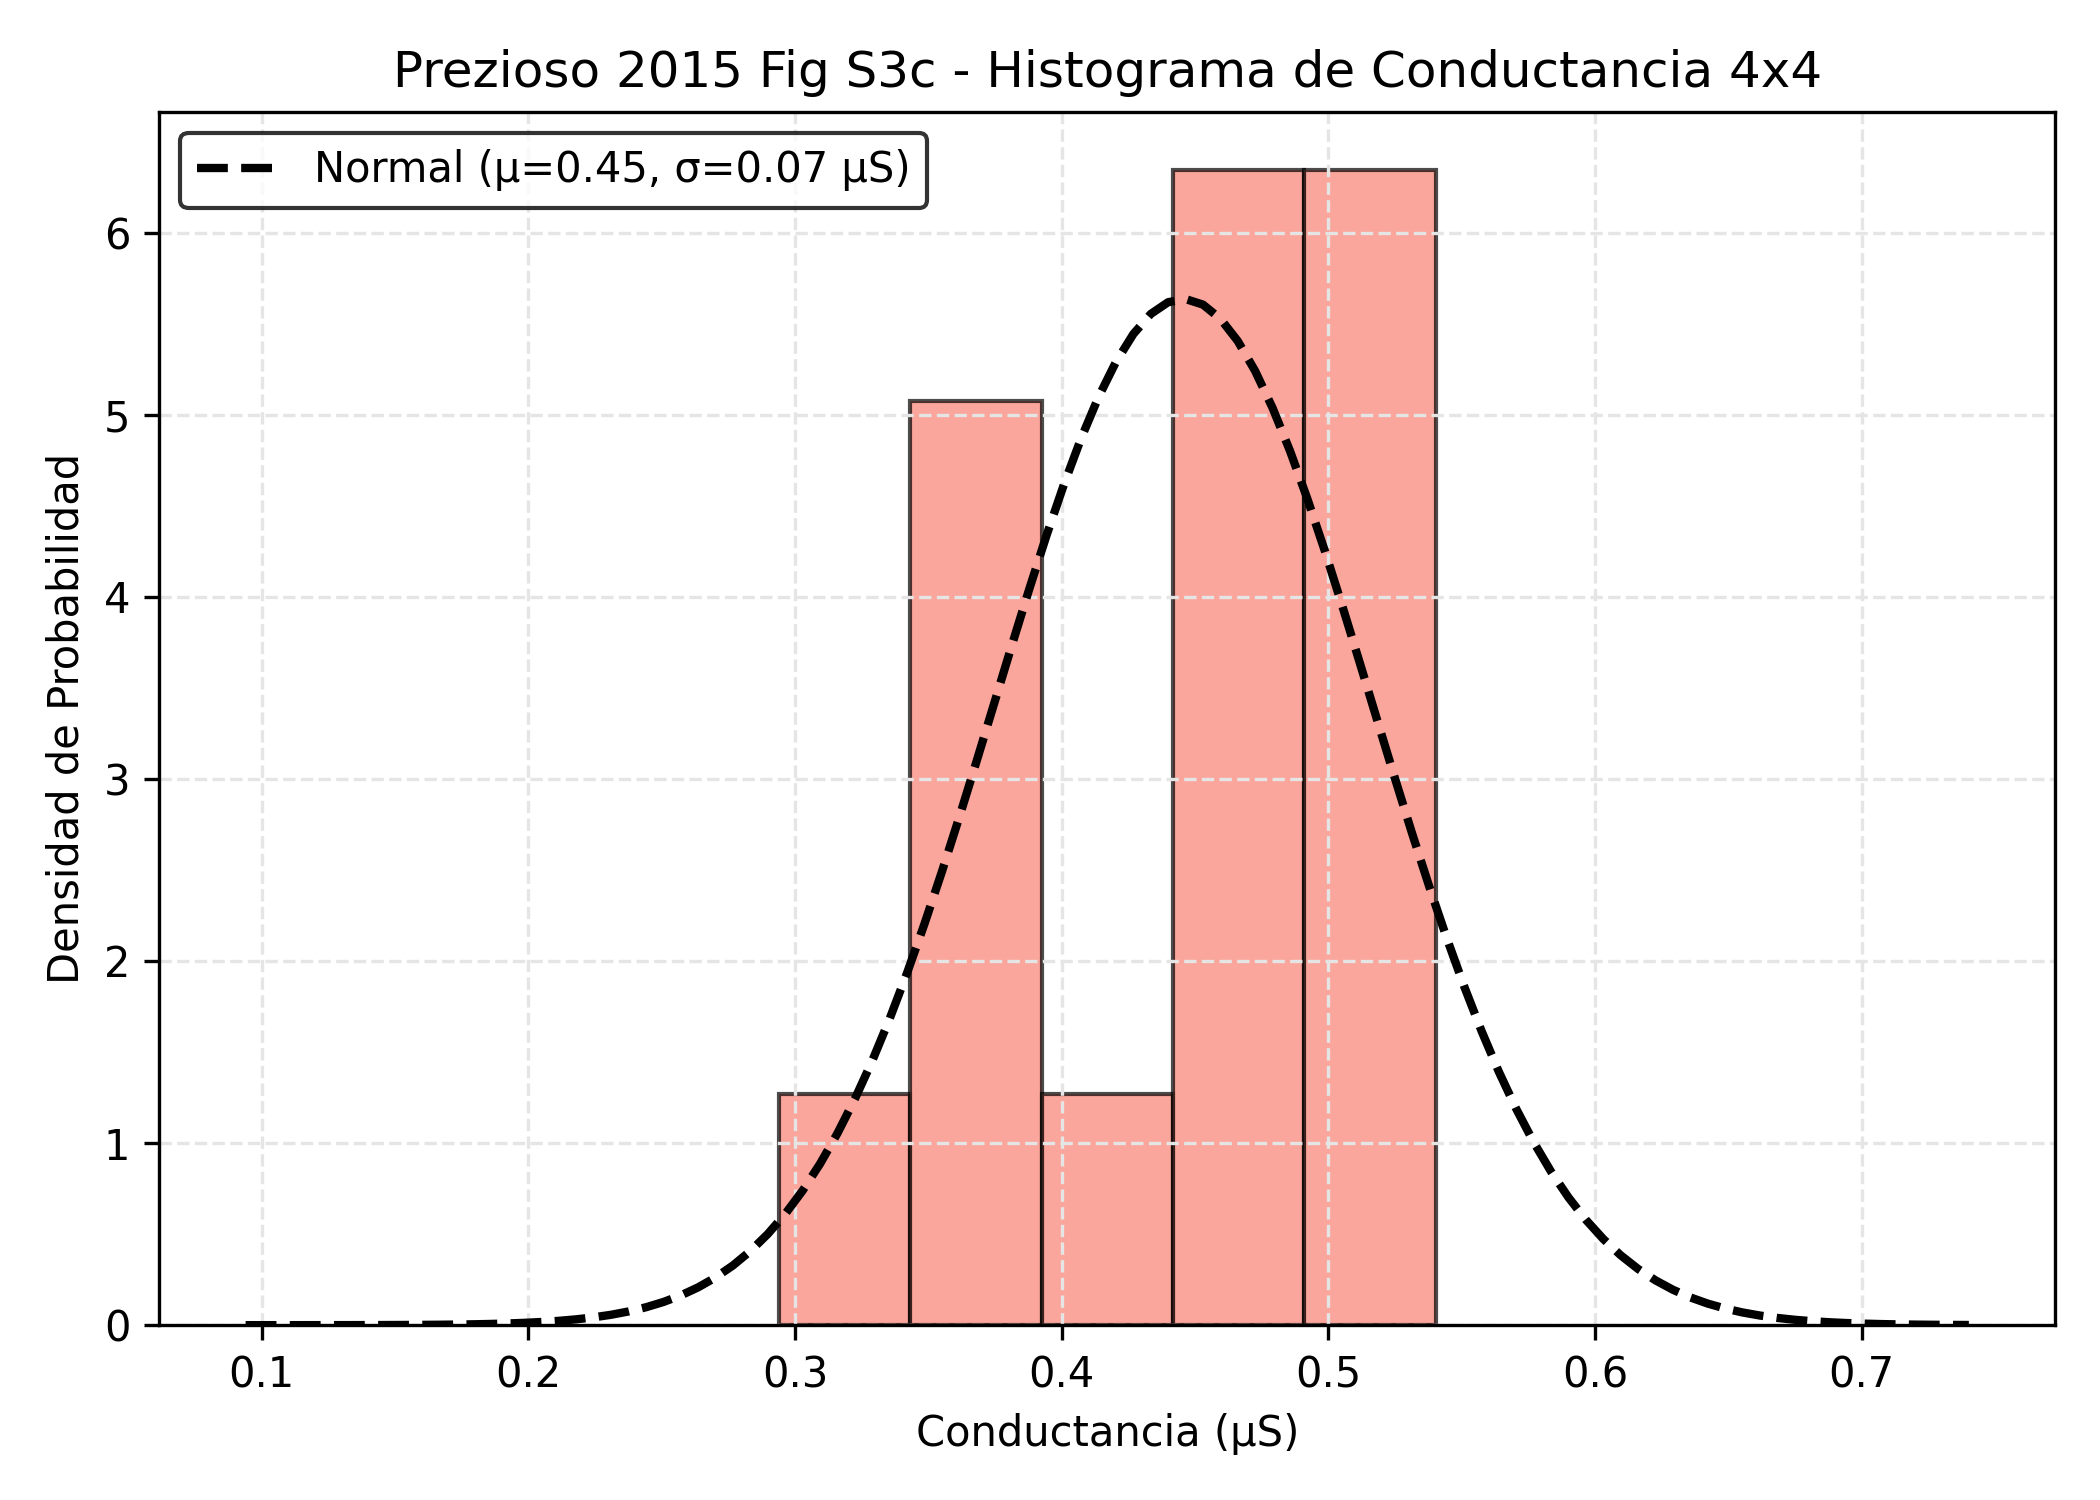
\includegraphics[width=\textwidth]{figuras/23c_prezioso_s3c.png}
        \caption{Análisis espectral y poblacional (D2D).}
    \end{subfigure}
    \caption{Mediciones cruzadas cuantitativas y estadísticas sobre la dispersión de red nativa, en alineación exhaustiva a S3b y S3c (Prezioso 2015).}
    \label{fig:prezioso_s3bc}
\end{figure}

\textbf{Propósito y Relevancia:} Representa la validación espacial y poblacional de la arquitectura a gran escala. El mapa de calor (Heatmap) y el histograma estadístico demuestran categóricamente que \texttt{neurolab} es capaz de instanciar un Crossbar entero (matriz $4 \times 4$) dotado con la misma varianza estocástica Device-to-Device (D2D) observada en el hardware físico reportado en la revista \textit{Nature}. Esto acredita que cualquier red neuronal entrenada en este simulador lidiará con los mismos niveles realistas de ruido espacial que un chip de silicio real.

\begin{figure}[H]
    \centering
    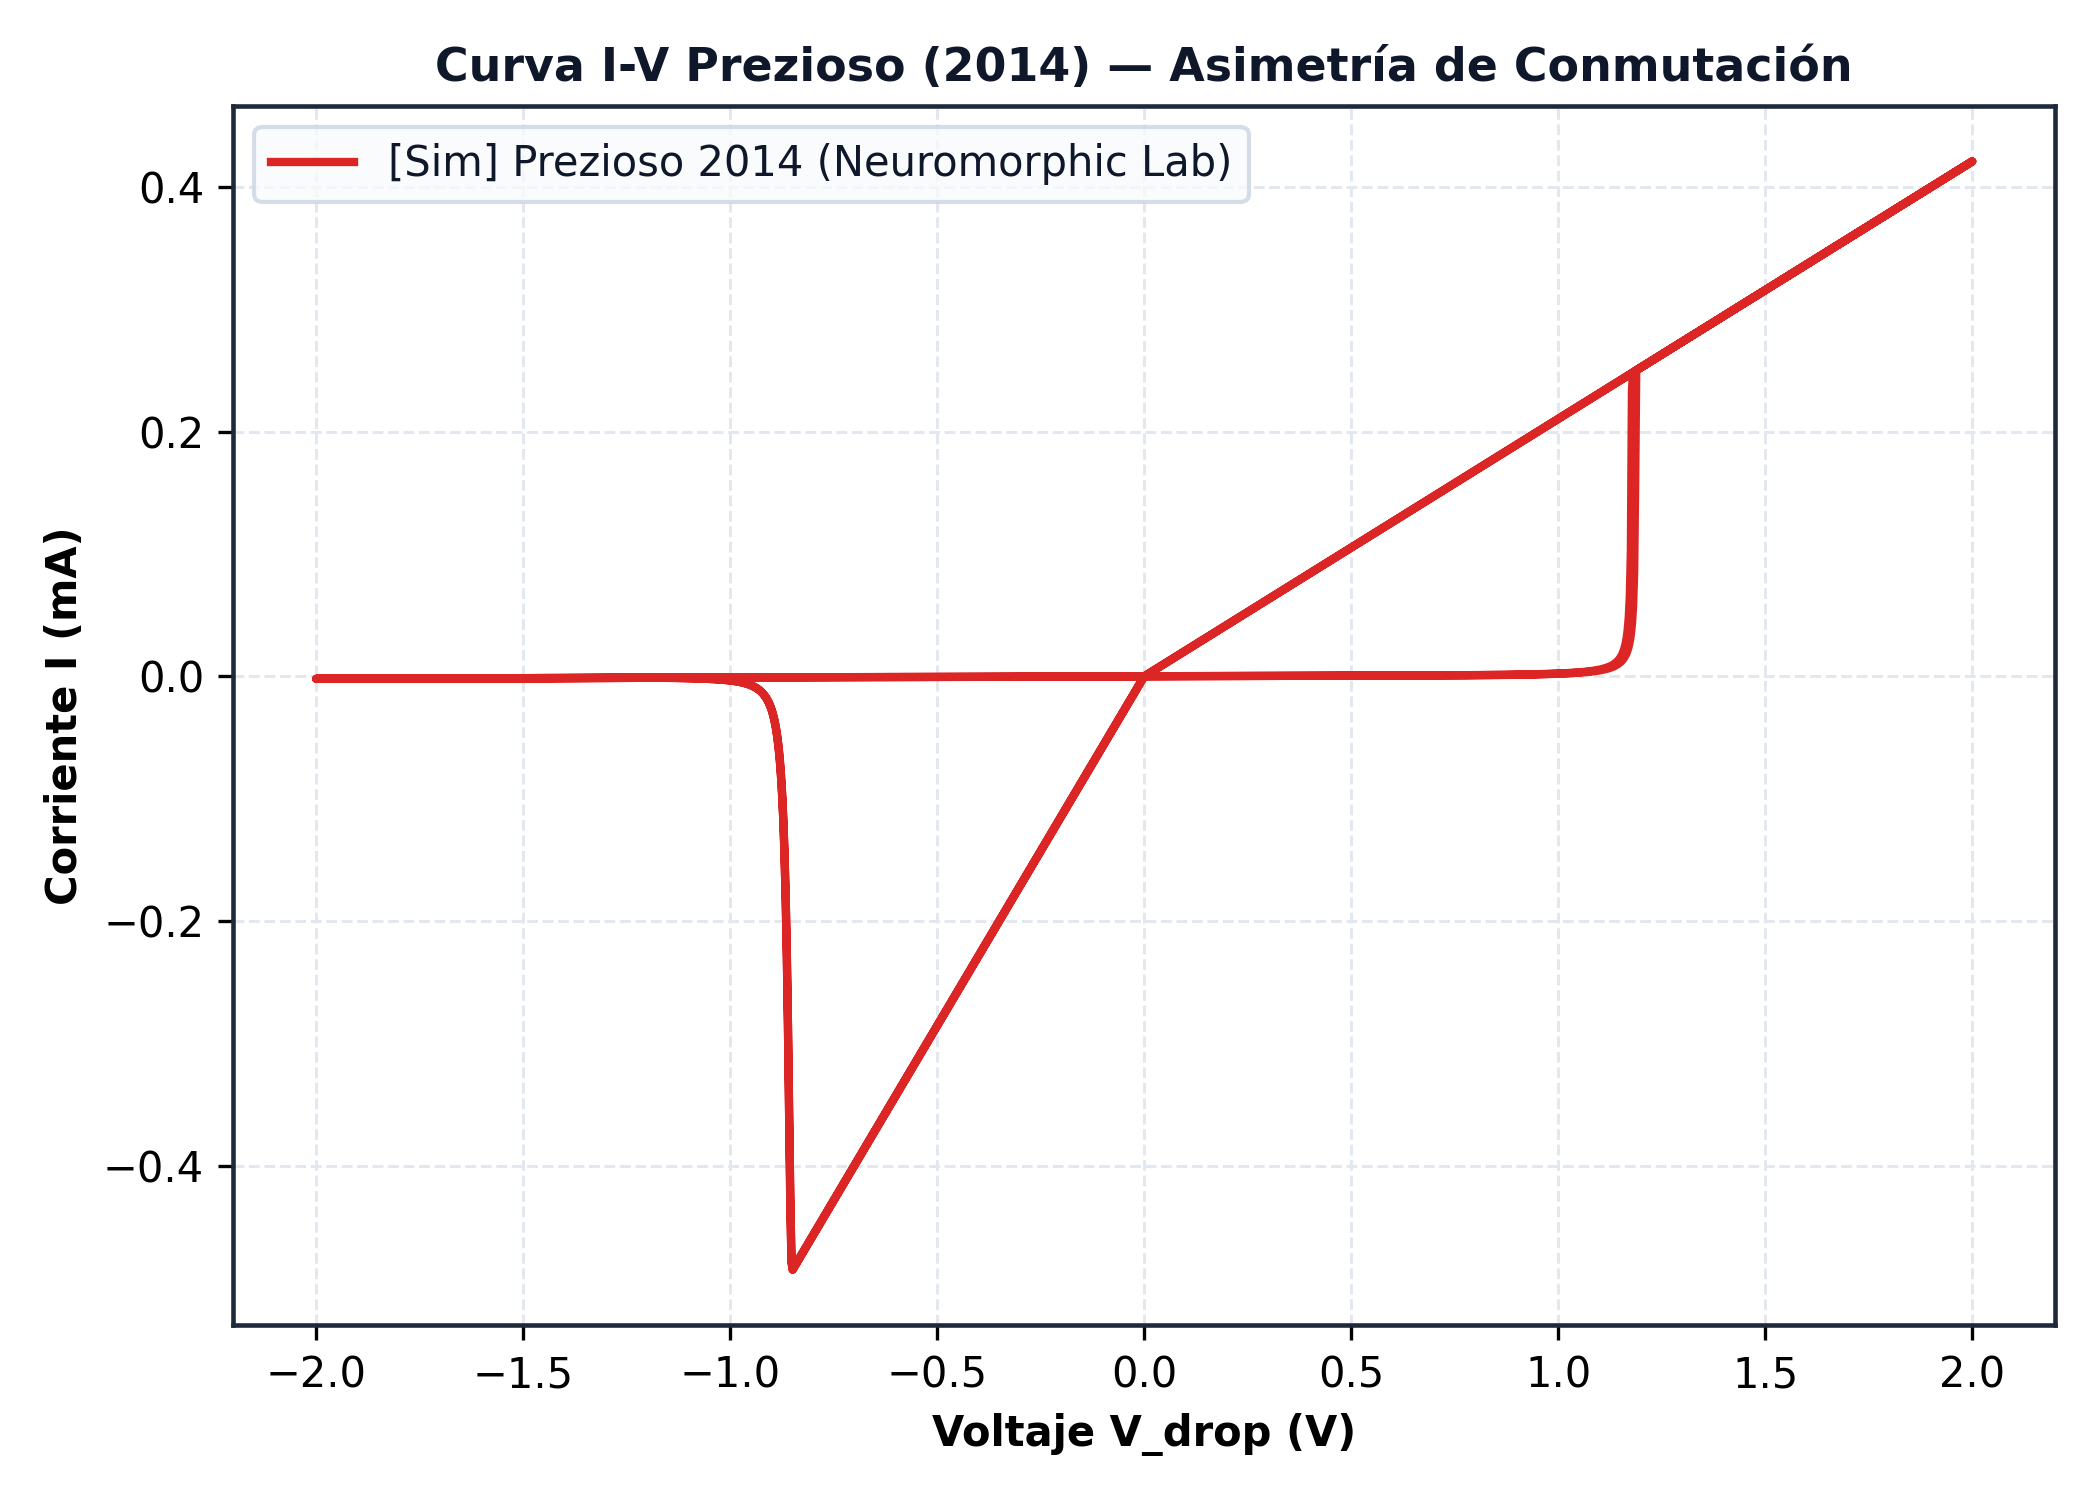
\includegraphics[width=0.7\textwidth]{figuras/fig_22_prezioso_v2.png}
    \caption{Validación de asimetría SET/RESET sobre la matriz en configuración Prezioso extendida.}
    \label{fig:22_prezioso_v2}
\end{figure}

\textbf{Propósito y Relevancia:} Funciona como la certificación definitiva a nivel de sistema cerrado. Verifica visualmente que cuando el modelo asimétrico Yakopcic/Prezioso se incrusta dentro de los nodos y restricciones resistivas de la matriz Crossbar compleja, sigue respondiendo perfectamente a las ventanas de operación SET/RESET. Garantiza que el escalamiento de memoria masiva no degrada ni corrompe las dinámicas analógicas subyacentes de los dispositivos atómicos.


